%!TEX TS-program = xelatex
%!TEX encoding = UTF-8 Unicode

\documentclass[12pt]{article}
\usepackage{geometry}                % See geometry.pdf to learn the layout options. There are lots.
\geometry{a4paper,top=2cm}
\usepackage[parfill]{parskip}    % Activate to begin paragraphs with an empty line rather than an indent
\usepackage{graphicx}
\usepackage{amsmath}
\usepackage{amssymb}
\usepackage{mathtools}
\usepackage{physics}
\newcommand{\be}{\begin{equation}}
\newcommand{\ee}{\end{equation}}
\usepackage[thicklines]{cancel}
\usepackage[colorlinks=true,citecolor=blue,linkcolor=blue,urlcolor=blue]{hyperref}
\usepackage{booktabs}
\usepackage{csquotes}
\usepackage{qcircuit}
\usepackage{circledsteps}
\usepackage{nicefrac}
\usepackage{fontspec,xltxtra,xunicode}
\usepackage{xcolor}
\usepackage{simplewick}
\defaultfontfeatures{Mapping=tex-text}

\newcommand{\polv}{\ensuremath{\updownarrow}}
\newcommand{\polh}{\ensuremath{\leftrightarrow}}
\newcommand{\poldr}{\rotatebox[origin=c]{45}{\ensuremath{\leftrightarrow}}}
\newcommand{\poldl}{\rotatebox[origin=c]{-45}{\ensuremath{\leftrightarrow}}}
\newcommand{\bigzero}{\mbox{\normalfont\Large\bfseries 0}}
\newcommand{\vecrp}{\ensuremath{\vec{r}^{\,\prime}}}
\newcommand{\vecnr}{\ensuremath{\vec{\nabla}_{\!r}}}

\title{Advanced Quantum Mechanics\\Class 28 (b)}
%\author{The Author}
\date{December 08, 2022}                                           % Activate to display a given date or no date

\begin{document}
\maketitle

\setcounter{section}{9}
\setcounter{subsection}{6}
\setcounter{equation}{136}

%%% 03 OKAY

\subsection{Inclusion of spin (continued)}

Remember the expression for the two-body potential:
\be
\begin{gathered}
V_2(k_1^\prime m_1^\prime, k_2^\prime m_2^\prime, k_1 m_1, k_2 m_2)
= 
\int d^3r\,d^3r^\prime
\phi^*_{k_1^\prime m_1^\prime}(\vec{r})
\phi^*_{k_2^\prime m_2^\prime}(\vecrp)\times\\
[V_2(\vec{r},\vecrp)]_{m_1^\prime m_2^\prime, m_1 m_2}
\phi_{k_2 m_2}(\vecrp)
\phi_{k_1 m_1}(\vec{r})
\end{gathered}
\label{eq:g137}
\ee

\emph{Suppose that:} $k$ represents momentum $\vec{k}$
\be
\phi_{km}(\vec{r})=\frac{1}{L^{3 / 2}} e^{i \vec{k} \cdot \vec{r}} \chi_{m}
\ee
\textit{i.e}, wave planes in a box,
%%% 04 OKAY
and
$V_{2}(\vec{r}, \vec{r}, s)=V_{2}\left(\vec{r}-\vecrp, s\right)$.
We will, as usual, assume periodic boundary conditions and take the $L \to \infty$ limit in the end.
Eq.~\eqref{eq:g137} can be written as
\be
\begin{gathered}
V_2(k_1^\prime m_1^\prime, k_2^\prime m_2^\prime, k_1 m_1, k_2 m_2)
= 
\int \frac{d^3r\,d^3r^\prime}{L^3}
\exp(-i\vec{k}_1^\prime\cdot\vec{r})
\exp(-i\vec{k}_2^\prime\cdot\vecrp)\\
[V_2(\vec{r}-\vecrp),s]_{m_1^\prime m_2^\prime, m_1 m_2}
\exp(-i\vec{k}_2       \cdot\vecrp)
\exp(-i\vec{k}_1       \cdot\vec{r})
\end{gathered}
\ee
%
\begin{enumerate}
\item change of variable:
\be 
\vec{r}-\vecrp = \vec{z}; \quad \vec{r} = \vecrp + \vec{z} 
\ee
%
\item exponentials can be rewritten as
\be
\begin{gathered}
\exp(-i(\vec{k}_1^\prime-\vec{k}_1)\cdot(\vecrp+\vec{z})
	 -i((\vec{k}_2^\prime-\vec{k}_2)\cdot\vecrp))\\
= \exp(-i(\vec{k}_1^\prime + \vec{k}_2^\prime 
		 -\vec{k}_1        - \vec{k}_2)\cdot\vecrp)
  \exp(-i(\vec{k}_1^\prime - \vec{k}_1)\cdot\vec{z})
\end{gathered}
\ee
%
\item integrate over $\vecrp$
\be
\frac{1}{L^3} \int d^3r^\prime
\exp(-i(\vec{k}_1^\prime + \vec{k}_2^\prime 
	   -\vec{k}_1        - \vec{k}_2)\cdot\vecrp)
= \delta_{\vec{k}_1^\prime + \vec{k}_2^\prime, \vec{k}_1+\vec{k}_2}	
\ee
where the delta is a Kronecker delta (we put the particle in a box),
and represents momentum conservation.
%
\item the remaining integral over $\vec{z}$ leads to the Fourier
transform of the potential
\be
\int d^3z \exp(-i(\vec{k}_1^\prime - \vec{k}_1)\cdot\vec{z})
V_2(\vec{z},s) = \widetilde{V}_2(\vec{k}_1^\prime - \vec{k}_1, s)
\ee
\end{enumerate}
%%% 05 OKAY
Putting all together, the equation for the second-quantized two-body interaction $\hat{V}_2$ becomes:
\be
\begin{gathered}
\hat{V}_2 = \frac{1}{2}
\sum_{m_1m_1^\prime}\sum_{m_2m_2^\prime}
\frac{1}{L^3} \delta_{\vec{k}_1^\prime + \vec{k}_2^\prime, \vec{k}_1+\vec{k}_2}
\sum_{k_1k_1^\prime}\sum_{k_2k_2^\prime}\\
\times
[\widetilde{V}_2(\vec{k}_1^\prime - \vec{k}_1, s)]_{m_1^\prime m_2^\prime, m_1 m_2}
\times 
\hat{a}_{k_1^\prime m_1^\prime}^{\dagger} \hat{a}_{k_2^\prime m_2^\prime}^{\dagger} 
\hat{a}_{k_2 m_2} \hat{a}_{k_1 m_1}
\end{gathered}
\label{eq:g144}
\ee

When $V_2$ is spin-independent,
\be
[\widetilde{V}_2(\vec{k}_1^\prime - \vec{k}_1, s)]_{m_1^\prime m_2^\prime, m_1 m_2}
=
\delta_{m_1^\prime m_1}\delta_{m_2^\prime,m_2}
\widetilde{V}_2(\vec{k}_1^\prime - \vec{k}_1)
\ee
then one can write for $\hat{V}_2$
\be
\begin{gathered}
\hat{V}_2 = \frac{1}{2}
\sum_{m_1m_2}
\frac{1}{L^3} \delta_{\vec{k}_1^\prime + \vec{k}_2^\prime, \vec{k}_1+\vec{k}_2}
\sum_{k_1k_1^\prime}\sum_{k_2k_2^\prime}\\
\times
\widetilde{V}_2(\vec{k}_1^\prime - \vec{k}_1)
\times 
\hat{a}_{k_1^\prime m_1}^{\dagger} \hat{a}_{k_2^\prime m_2}^{\dagger} 
\hat{a}_{k_2 m_2} \hat{a}_{k_1 m_1}
\end{gathered}
\label{eq:g146}
\ee

One can eliminate the momentum-conserving delta
function in Eqs.~\eqref{eq:g144} and \eqref{eq:g146} by integrating \textit{e.g.}
over $\vec{k}_{2}^{\prime}$, so that $\vec{k}_{2}^{\prime}=\vec{k}_{1}+\vec{k}_{2}-\vec{k}_{1}^{\prime}$. Defining
\be
\vec{q} = \vec{k}_{1}^{\prime}-\vec{k}_{1}
\ee
and renaming $\vec{k}_{1} \to \vec{k}$, $\vec{k}_{2} \to \vec{p}$, one has
\be
\vec{k}_{1}^{\prime} = \vec{q}+\vec{k}_{1} = 
\vec{k}+\vec{q},\quad
\vec{k}_{2}^{\prime} = \vec{k}_{1}+\vec{k}_{2} - \vec{k}_{1}^{\prime} =
\vec{p}+\vec{q}
\ee
%%% 06 OKAY
and $\hat{V}_2$ can be rewritten as
\be
\hat{V}_2 = \frac{1}{2L^3}
\sum_{kpq} \sum_{mm^\prime}
\widetilde{V}_2(\vec{q})
\hat{a}^\dagger_{k+q,m} \hat{a}^\dagger_{p+q, m^{\prime}} 
\hat{a}_{p, m^{\prime}} \hat{a}_{k,m}
\ee

\emph{Pictorial view of $\widetilde{V}_2$}: transition from an initial state
$\ket{i} = \hat{a}^\dagger_{k_1m_1}\hat{a}^\dagger_{k_2m_2}\ket{0}$
to a final state
$\ket{f} = \hat{a}^\dagger_{k_1^\prime m_1^\prime }\hat{a}^\dagger_{k_2^\prime m_2^\prime }\ket{0}$.

The matrix element $\bra{f}\hat{V}_2\ket{i}$ is given by:
%%% The gigantic calculation...
\[
\begin{gathered}
\bra{f}\hat{V}_2\ket{i} = 
\bra{0}\hat{a}_{k_2^\prime m_2^\prime}\hat{a}_{k_1^\prime m_1^\prime}
|\hat{V}_2|
\hat{a}^\dagger_{k_1m_1}\hat{a}^\dagger_{k_2m_2}\ket{0}\\
=
\frac{1}{2L^3}\sum_q \widetilde{V}_2(\vec{q}) \sum_{kp,mm^\prime}
\bra{0}\hat{a}_{k_2^\prime m_2^\prime}\hat{a}_{k_1^\prime m_1^\prime}
\hat{a}^\dagger_{k+q,m} \hat{a}^\dagger_{p+q, m^{\prime}} 
%\times
\hat{a}_{p, m^{\prime}} \hat{a}_{k,m}
\hat{a}^\dagger_{k_1m_1}\hat{a}^\dagger_{k_2m_2}\ket{0}
\end{gathered}
\]
%
\[
\begin{gathered}
=
\frac{1}{2L^3}\sum_q \widetilde{V}_2(\vec{q}) \sum_{kp,mm^\prime}
\bra{0}\hat{a}_{k_2^\prime m_2^\prime}\hat{a}_{k_1^\prime m_1^\prime}
\hat{a}^\dagger_{k+q,m} \hat{a}^\dagger_{p+q, m^{\prime}}\ket{0}\\
\left(
	\delta_{k k_{1}} \delta_{k k_{2}} \delta_{m m_{1}} \delta_{m^{\prime} m_{2}} \pm 
	\delta_{k k_{2}} \delta_{p k_{1}} \delta_{m m_{2}} \delta_{m^{\prime} m_{1}}
	\right)
\end{gathered}
\]
%
\[
\begin{gathered}
=
\frac{1}{2L^3}\sum_q \widetilde{V}_2(\vec{q}) \sum_{kp,mm^\prime}
\big(
	\delta_{k+q, k_{1}^{\prime}} \delta_{p-q, k_{2}^{\prime}} \delta_{m m_{1}^{\prime}} \delta_{m^{\prime} m_{2}^{\prime}}
\\
\pm	\delta_{k+q, k_{2}^{\prime}} \delta_{p-q, k_{1}^{\prime}} \delta_{m m_{2}}^{\prime} \delta_{m^{\prime} m_{1}^{\prime}}
\big)
\times
\left(
	\delta_{k k_{1}} \delta_{k k_{2}} \delta_{m m_{1}} \delta_{m^{\prime} m_{2}} \pm 
	\delta_{k k_{2}} \delta_{p k_{1}} \delta_{m m_{2}} \delta_{m^{\prime} m_{1}}
	\right)
\end{gathered}
\]
%%% 07
\[
=\frac{1}{L^3}
\delta_{k_{1}+k_{2}, k_{1}^{\prime} + k_{2}^{\prime}}
\sum_q \widetilde{V}_2(\vec{q})
\left(
\delta_{m_{1}^{\prime} m_{1}}\delta_{m_{2}^{\prime} m_{2}}\delta_{q,k_{1}^{\prime}-k_{1}}
\pm
\delta_{m_{1}^{\prime} m_{2}}\delta_{m_{2}^{\prime} m_{1}}\delta_{q,k_{1}^{\prime}-k_{2}}
\right)
\]
so finally, using the deltas that involves $\vec{q}$,
\be
\begin{gathered}
\bra{f}\hat{V}_2\ket{i} = 
\delta_{k_{1}+k_{2}, k_{1}^{\prime} + k_{2}^{\prime}}
\left[
\widetilde{V}_2(k_{1}^{\prime}-k_{1})\delta_{m_{1}^{\prime} m_{1}}\delta_{m_{2}^{\prime} m_{2}}
\pm
\widetilde{V}_2(k_{1}^{\prime}-k_{2})\delta_{m_{1}^{\prime} m_{2}}\delta_{m_{2}^{\prime} m_{1}}
\right]\\
\Rightarrow \text{rewriting }
\delta_{k_{1}+k_{2}, k_{1}^{\prime} + k_{2}^{\prime}}
=
\delta_{k_{1}^{\prime} - k_{1}, k_{2} - k_{2}^{\prime}}
\end{gathered}
\label{eq:g150}
\ee
The first term in \eqref{eq:g150} is the ``direct'' term, while the second one is the ``exchange''. They can be visualised like this (direct on the left, exchange on the right):
\begin{center}
\includegraphics[width=0.45\textwidth]{Figures/direct.pdf}
\hfill
\includegraphics[width=0.45\textwidth]{Figures/exchange.pdf}
\end{center}
where in the $\pm$ sign, the $+$ is for bosons and the $-$ is for fermions.
At each vertice, momentum is conserved.

%%% 08 OKAY

One can simplify a lot the notation if one lumps
together orbital and spin quantum numbers into
a single index: $k m \equiv \alpha$. When $k \rightarrow \vec{k}, \alpha=\vec{k} m$.
When $k$ refers to energy states in a spherically
symmetric potential, they are charaterized by several
quantum numbers, \textit{e.g}. $nlsjm$, so that
\be
\hat{a}_{k m}=\hat{a}_{n l s j m} \equiv \hat{a}_{\alpha}
\ee
In either case, the (anti) commutation relations are summari-
zed by:
\be
\left[\hat{a}_{\alpha}, \hat{a}_{\beta}\right]_{\mp}=0,\quad
\left[\hat{a}_{\alpha}, \hat{a}_{\beta}\right]_{\mp}=\delta_{\alpha \beta}
\ee
The Hamiltonian, containing one- and two-body
interactions is then written as
\be
\hat{H}_{2}=\sum_{\alpha \beta} \langle\alpha|H_{1}| \beta\rangle \hat{a}_{\alpha}^\dagger\hat{a}_{\beta}
+ \frac{1}{2}
\sum_{\alpha \beta \gamma \delta} V(\alpha \beta, \gamma \delta) \hat{a}_{\alpha}^{\dagger} \hat{a}_{\beta}^{\dagger} \hat{a}_{\delta} \hat{a}_{\gamma}
\ee

%%% 09 (just the part we need)

\subsection{Applications}

\subsubsection{Noninteracting Fermi gas in a box}

(We assume all the first quantization results are known.)

\emph{Pauli principle:} $(2s+1) = g$ particles per momentum state.
Ground state: occupy all lowest single particle energies
consistent with the Pauli principle.
The maximum momentum $\vec{k}_\text{max}$ is the Fermi momentum $k_F$.
\begin{center}
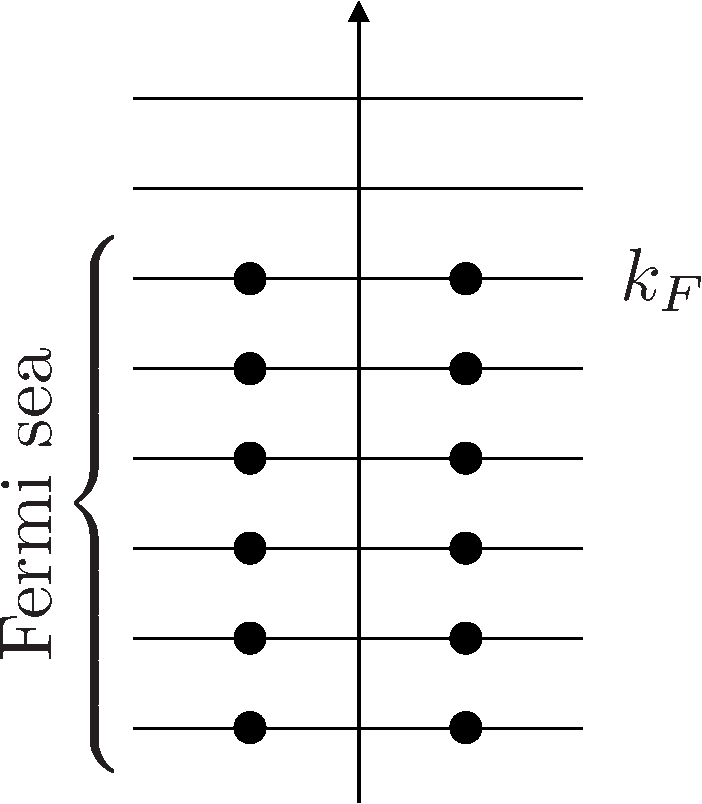
\includegraphics[width=0.3\textwidth]{Figures/FermiSea.pdf}
\end{center}

%%% 11 OKAY

\emph{Second quantization}: appropriate basis $\{\hat{a}_{k m}, \hat{a}^\dagger_{k m}\}$.

The Fock-space Hamiltonian of the noninteracting system
is given by Eq.~(135) with $V_{1}=0$ and $\varepsilon_{k m}=\frac{\hbar^{2} k^{2}}{2 M}$:
\setcounter{equation}{159}
\be
\hat{H}=\sum_{m} \sum_{k} 
\frac{\hbar^{2} k^{2}}{2 M} \hat{a}^\dagger_{k m} \hat{a}_{k m}
\ee
Here it pays off to use $\vec{k}m = \alpha$:
\be
\varepsilon_{\alpha} \equiv \frac{\hbar^{2} \vec{k}^{2}}{2 M}
\ee
\be
\hat{H}=\sum_{\alpha} \varepsilon_{\alpha} \hat{a}_{\alpha}^{\dagger} \hat{a}_{\alpha}=\sum_{a} \varepsilon_{\alpha} \hat{N}_{\alpha}
\ee
with
\be
\hat{N}_\alpha = \hat{a}_{\alpha}^{\dagger} \hat{a}_{\alpha}
\ee

In this notation, the ground state $\left|\Psi_{0}\right\rangle$ can be
written as
\be
\begin{aligned}
\left|\Psi_{0}\right\rangle
&=a_{k_{1}-s}^{\dagger} \ldots \hat{a}_{k_{1} s}^{\dagger} \hat{a}_{k_{2}-s}^{\dagger} \ldots \hat{a}_{k_{2} s} \ldots \ldots \hat{a}_{k_{F} s}^{\dagger}|0\rangle\\
&=\prod_{m} \prod_{k}^{k_{F}} \hat{a}_{km}^{\dagger}|0\rangle
=\prod_{a}^{\alpha_{\text {max}}} \hat{a}_{\alpha}^{\dagger} |0\rangle
\end{aligned}
\label{eq:g164}
\ee
where $\alpha_{\text {max}}$ is to be understood as relating to the
momentum $k_{F}$ and spin projection $+s$.

%%% 12 OKAY

The ground-state density is $\rho=N / V$, where $N$ is the expectation
value of the number operator $\hat{N}$ in the state $\left|\Psi_{0}\right\rangle$:
\be
N=\left\langle\Psi_{0}|\hat{N}| \Psi_{0}\right\rangle=\sum_{\alpha}\left\langle\Psi_{0}\left|\hat{a}^\dagger_{\alpha} \hat{a}_{\alpha}\right| \Psi_{0}\right\rangle
\ee
Easy way to evaluate the matrix element:
\[
\left\langle\Psi_{0}\left|\hat{a}^\dagger_{\alpha} \hat{a}_{\alpha}\right| \Psi_{0}\right\rangle = 
\langle\Psi_{0}|\hat{a}^\dagger_{\alpha} 
\underbrace{\hat{a}_{\alpha}\hat{a}^\dagger_{\alpha_1}\ldots\hat{a}^\dagger_{\alpha_{\text {max}}} \ket{0}}%
_{\Circled{1}}
\]
where \Circled{1} is a
state with a ``hole'' in
the Fermi sea at some
$\alpha_{a}$ -- this is similar
to the result in
Eq.~(46) first line.
$\hat{a}_{\alpha}^\dagger$ must fill that hole
so that $\ket{\Psi_{0}}$ is recovered,
otherwise $\left\langle\Psi_{0} | \cdots\right\rangle=0$.
So you make that assumption, and it gives $\bra{\Psi_0}\ket{\Psi_0} = 1$.
Therefore
\be
\begin{aligned}
N
&=\sum_{\alpha}\left\langle\Psi_{0}\left|\hat{a}_{\alpha}^{\dagger} a_{\alpha}\right| \Psi_{0}\right\rangle=\sum_{\alpha}^{\alpha_{\text {max}}} 1\\
&= \sum_{m} \sum_{\hbar}^{k_{F}} 1=g \sum_{k}^{k_{F}} 1\\
&= g \frac{L^3}{8 \pi^{3}} \int d^{3} k \,\theta\!\left(k_{F}-\left|\vec{k}\right|\right) = 
g \frac{L^3}{8 \pi^{3}}  \frac{4 \pi}{3}k_{F}^{3}\\
& = \frac{gL^3}{6 \pi^{2}} k_{F}^{3} \Rightarrow \rho = \frac{N}{V} 
= \frac{g}{6 \pi^{2}} k_{F}^{3}\,\checkmark
\end{aligned}
\ee

%%% 13 OKAY

The calculation of the energy is similar to this
\be
\begin{aligned}
E
&=\left\langle\Psi_{0}|\hat{H}| \Psi_{0}\right\rangle
=\sum_{m} \sum_{k} \frac{\hbar^{2} \vec{k}^{2}}{2 M}
\underbrace{\left\langle\Psi_{0}\left|\hat{a}^\dagger_{k m} \hat{a}_{k m}\right| \Psi_{0}\right\rangle}%
_{\text{same as above}}\\
&=g \frac{L}{8 \pi^{3}} \frac{\hbar^{2}}{2 M} 4 \pi \int_{0}^{k_{F}} d k k^{4}
\end{aligned}
\ee
This leads to the same results
for $\varepsilon = E/V$, $E/N$ and $P$ (pressure) given
by the first quantization technique.

\subsubsection{Effects of an interaction}

Interacting \emph{Fermi} gas:
\be
\hat{V}_{2}=1 / 2 \sum V_{\alpha \beta \gamma \delta}(\alpha \beta, \gamma \delta) \hat{a}_{\alpha}^{\dagger} \hat{a}_{\beta}^{\dagger} \hat{a}_{\delta} \hat{a}_{\gamma}
\ee
We will use first-order perturbation theory: the
zeroth order approximation is the ground state $\left|\Psi_{0}\right\rangle$
of the noninteracting Fermi gas, Eq.~\eqref{eq:g164}. The first order
correction to the energy is
\be
E^{(1)}=\left\langle\Psi_{0}\left|\hat{V}_{2}\right| \Psi_{0}\right\rangle
\ee

%%% 14 OKAY

The calculation of the matrix element can be made
as follows. First, note that when $\hat{V}_{2}$ acts on
$\left|\Psi_{0}\right\rangle$, the product $\hat{a}_{\delta} \hat{a}_{\gamma}$ digs two holes in the
Fermi sea; this means that the product $\hat{a}_{\alpha}^\dagger\hat{a}_{\beta}\dagger$
has to fill up those holes so that $\left|\Psi_{0}\right\rangle$ is recovered.

\emph{Note that}:
\begin{enumerate}
\item In the process of digging two holes, there might
be a $(-1)$ due to the anticommutating nature
of the $\hat{a}$ and $\hat{a}^{\dagger}$ operators:
\be
\ket{\alpha_1\alpha_2\ldots\alpha_{a-1}\,{}_\text{(hole)}\,\alpha_{a+1}
\ldots
\alpha_{b-1}\,{}_\text{(hole)}\,\alpha_{b+1}
\ldots
\alpha_{\text{max}}
}
\ee
$(-1)$ if $\hat{a}_{\delta} \hat{a}_{\gamma}$ have jumped over an
odd number of operators.
%
\item Such a $(-1)$ is cancelled by another $(-1)$
due to the $\hat{a}_{\alpha}^{\dagger} \hat{a}_{\beta}^{\dagger}$, since they must jump
over number of operators that $\hat{a}_{\delta} \hat{a}_{\gamma}$ have.
\begin{itemize}
\item This is true if this happens in the
``direct'' order
\[
\contraction[1.5ex]{}%
{\hat{a}_{\alpha}^{\dagger}}%
{\hat{a}_{\beta}^{\dagger}\hat{a}_{\delta}}%
{\hat{a}_{\gamma}}%%%
\contraction%
{\hat{a}_{\alpha}^{\dagger}}%
{\hat{a}_{\beta}^{\dagger}}{}{\hat{a}_{\delta}}%
{\hat{a}_{\alpha}^{\dagger}}%
{\hat{a}_{\beta}^{\dagger}\hat{a}_{\delta}}%
{\hat{a}_{\gamma}}
\]
meaning that
%%% 15 OKAY
$\hat{a}^\dagger_{\beta}$ fills the hole dug by $\hat{a}_{\delta}$ and
$\hat{a}^\dagger_{\alpha}$ fills the hole dug by $\hat{a}_{\gamma}$.
\item The ``exchange'' order is the nve in which
$\hat{a}^\dagger_{\beta}$ fills the hole dug by $\hat{a}_{\gamma}$ and
$\hat{a}^\dagger_{\alpha}$ fills the hole dug by $\hat{a}_{\delta}$.
In this case, there is a relative
$(-1)$ between the two contriburions.
\end{itemize}
\end{enumerate}
In summary, the matrix element is given by
\be
E^{(1)}=\frac{1}{2} \sum_{\alpha \beta}^{k_{F}}\left[V_{2}(\alpha \beta, \alpha \beta)-V_{2}(\alpha \beta, \beta \alpha)\right]
\ee

For a spin-independent $V_{2}$, one can use the result in
in Eq.~\eqref{eq:g150} to obtain
\be
\begin{gathered}
E^{(1)}=\frac{1}{2 L^{3}} \sum_{k_{\alpha}}^{k_{F}} \sum_{k_{\beta}}^{k_{F}} \delta_{\vec{k}_{\alpha}+\vec{k}_{\beta}-\vec{k}_{\alpha}-\vec{k}_{\beta}} \sum_{m_{\alpha} m_{\beta}}
\times\\
\left\{
 \delta_{m_{\alpha} m_{\alpha}} \delta_{m_{\beta} m_{\beta}} \widetilde{V}_{2}(0)
-\delta_{m_{\alpha} m_{\beta}} \widetilde{V}_{2}\left(\vec{k}_{\alpha}-\vec{k}_{\beta}\right)
\right\}
\end{gathered}
\ee
%%% 16 OKAY, the part we need
One can now take the $L \to \infty$ limit to obtain
\be
\begin{gathered}
E^{(1)}=\frac{1}{2 L^{3}}\left(\frac{L^{3}}{8 \pi^{3}}\right)^{2}\bigg[g^{2} \int^{k_{F}} d^{3} k_{\alpha} \int^{k_{F}} d^{3} k_{\beta} \,\widetilde{V}_{2}(0)\\
-g \int^{k_{F}} d^{3} k_{\alpha} \int^{k_{F}} d^{3} k_{\beta} \,\widetilde{V}\left(\vec{k}_{\alpha}-\vec{k}_{\beta}\right)\bigg]
\end{gathered}
\ee
%%% 17 OKAY
Solving this integral, and supposing $V_2(\vec{r}) = V_2(r)$ (spherically symmetric) for simplicity, will lead us to
\setcounter{equation}{175}
\be
\boxed{
\frac{E^{(1)}}{L^{3}}=\frac{1}{2} \rho^{2} \int d^{3} r\, V_{2}(r)\left[1-\frac{9}{g}
\left(\frac{j_{1}\left(k_{F} r\right)}{\left(k_{F} r\right)^{2}}\right)^{2}\right]
}
\ee

The total energy densify per particle of the system, in
this approximation, is then given by
\be
\boxed{
\frac{E}{N}=\frac{3}{5} E_{F}+
\frac{1}{2} \rho \int d^{3} r \, V_{2}(r)
\left[1-\left(\frac{j_{1}\left(k_{F} r\right)}{k_{F} r}\right)^{2}\right]
}
\label{eq:g177}
\ee
where the first term  in between brackets (the 1) is from the direct interaction and the square involving the spherical Bessel function $j_1(k_F r)$ is from the exchange interaction.

%%% 18 OKAY

Note that the above result can be viewed as a
variational estimate of the exact ground state energy
(per particle) with $\rho$ (or $k_{F}$) being the variational
parameter:
\begin{itemize}
\item the expression involves the expectation value
of the Hamiltonian in the independent-particle
ansatz-state $\left|\psi_{0}\right\rangle$, which is parametrized
by the density $\rho$ (or, equivelently, by $k_F$).
\end{itemize}

For $V_{2}(r)<0$ (strictly attractive), it is easy to
see that Eq~\eqref{eq:g177} has no finite absolute
minimum for $\rho \neq 0$ : $E_{F} \sim \rho^{2 / 3}$ and the second
term $\sim-\rho$ (since the direct term dominates over
the exchange term, $j_{1}(k_{F} r) / k_{F} r$ oscillates wildly and
goes to zero as $k_{F}$ increases).
$\Rightarrow$ In this approximation, the system has no ground state! A better approximation is needed, but that is to be seen in an advanced solid state physics course.

\medskip

\begin{center}
\textbf{THE END}
\end{center}

\end{document}




















